%%%%%%%%%%%%%%%%%%%%%%%%%%%%%%%%%%%%%%%%%
% Beamer Presentation
% LaTeX Template
% Version 1.0 (10/11/12)
%
% This template has been downloaded from:
% http://www.LaTeXTemplates.com
%
% License:
% CC BY-NC-SA 3.0 (http://creativecommons.org/licenses/by-nc-sa/3.0/)
%
%%%%%%%%%%%%%%%%%%%%%%%%%%%%%%%%%%%%%%%%%

%----------------------------------------------------------------------------------------
%	PACKAGES AND THEMES
%----------------------------------------------------------------------------------------

\documentclass{beamer}
\setbeamertemplate{navigation symbols}{} % comment this out to ADD navigation tools

\usepackage{sansmathaccent}
\pdfmapfile{+sansmathaccent.map}

\mode<presentation> {

% The Beamer class comes with a number of default slide themes
% which change the colors and layouts of slides. Below this is a list
% of all the themes, uncomment each in turn to see what they look like.

%\usetheme{default}
%\usetheme{AnnArbor}
%\usetheme{Antibes}
%\usetheme{Bergen}
%\usetheme{Berkeley}
%\usetheme{Berlin}
%\usetheme{Boadilla}
%\usetheme{CambridgeUS}
%\usetheme{Copenhagen}
%\usetheme{Darmstadt}
%\usetheme{Dresden}
%\usetheme{Frankfurt}
%\usetheme{Goettingen}
%\usetheme{Hannover}
%\usetheme{Ilmenau}
%\usetheme{JuanLesPins}
%\usetheme{Luebeck}
%\usetheme{Madrid}
%\usetheme{Malmoe}
%\usetheme{Marburg}
%\usetheme{Montpellier}
%\usetheme{PaloAlto}
%\usetheme{Pittsburgh}
%\usetheme{Rochester}
%\usetheme{Singapore}
\usetheme{Szeged}
%\usetheme{Warsaw}

% As well as themes, the Beamer class has a number of color themes
% for any slide theme. Uncomment each of these in turn to see how it
% changes the colors of your current slide theme.

%\usecolortheme{albatross}
\usecolortheme{beaver}
%\usecolortheme{beetle}
%\usecolortheme{crane}
%\usecolortheme{dolphin}
%\usecolortheme{dove}
%\usecolortheme{fly}
%\usecolortheme{lily}
%\usecolortheme{orchid}
%\usecolortheme{rose}
%\usecolortheme{seagull}
%\usecolortheme{seahorse}
%\usecolortheme{whale}
%\usecolortheme{wolverine}

%\setbeamertemplate{footline} % To remove the footer line in all slides uncomment this line
%\setbeamertemplate{footline}[page number] % To replace the footer line in all slides with a simple slide count uncomment this line

%\setbeamertemplate{navigation symbols}{} % To remove the navigation symbols from the bottom of all slides uncomment this line
}

\usepackage{graphicx} % Allows including images
\usepackage{booktabs} % Allows the use of \toprule, \midrule and \bottomrule in tables
\usepackage{amssymb}
\usepackage{amsmath}
\usepackage{array}
\usepackage{longtable}
\usepackage{everysel}
\usepackage{xtab}
\usepackage{ragged2e}
\usepackage[labelfont=bf]{caption}
\usepackage{url}
\usepackage{datetime}
\usepackage{setspace}
\usepackage{multicol}
\usepackage{vwcol}
\usepackage{caption}
\usepackage{subcaption}

% texpos setup for placing text or images anywhere on the page
\usepackage[absolute,overlay]{textpos}
\setlength{\TPHorizModule}{30mm}
\setlength{\TPVertModule}{\TPHorizModule}
\textblockorigin{10mm}{10mm} % start everything near the top-left corner

% line spacing options
%\singlespacing
%\onehalfspacing
%\doublespacing
\setstretch{1.3} % for custom spacing


%---------------------------------------------------------------------------
%	TITLE PAGE
%---------------------------------------------------------------------------

\title[Predicting Atom Location Using Machine Learning Algorithms]{Predicting Atom Location Using \\ Machine Learning Algorithms} % The short title appears at the bottom of every slide, the full title is only on the title page

\author{Adam Martini, Ran Tian, Wes Erickson} % your name
\institute[UO] % Your institution as it will appear on the bottom of every slide, may be shorthand to save space
{
University of Oregon \\ % Your institution for the title page
\medskip
\textit{martini@cs.uoregon.edu\\} % Your email address
\textit{jmty0083@cs.uoregon.edu\\}
\textit{wwe@uoregon.edu}
}

\newdate{date}{13}{6}{2014}
\date{\displaydate{date}} % Date, can be changed to a custom date

\begin{document}

\begin{frame}
\titlepage % Print the title page as the first slide
\end{frame}

%\begin{frame}
%\frametitle{Overview} % Table of contents slide, comment this block out to remove it
%\tableofcontents % Throughout your presentation, if you choose to use \section{} and \subsection{} commands, these will automatically be printed on this slide as an overview of your presentation
%\end{frame}

%I suggest that you focus on the main points including the following:
%- what is the context of your work and why it is important? (one slide)
%
%- what are the key questions that you are exploring in your paper? (one slide)
%
%- what is the method/approach you used to organize selected studies (i.e. what are the 
%main aspects/metrics/issues you chose to compare and contrast different approaches, 
%in short what criteria you use to organize prior approaches in your report)
%is this your own method or you borrowed it from other places? (one slide)
%
%- What are the main points, findings, lessons learned in an organized (point by point) manner,
%again did you drive these points yourself or they are stated in other studies? (a few slides)

%----------------------------------------------------------------------------------------
%	PRESENTATION SLIDES
%----------------------------------------------------------------------------------------

%------------------------------------------------
%\section{Introduction} % Sections can be created in order to organize your presentation into discrete blocks, all sections and subsections are automatically printed in the table of contents as an overview of the talk
%------------------------------------------------

\section{Background} % A subsection can be created just before a set of slides with a common theme to further break down your presentation into chunks
% 1

\begin{frame}

\begin{itemize}
\item Why atom location?
	\begin{itemize}
	\item Camera in the Steck Lab takes pictures of atoms, but we want to know where its location.
	\end{itemize}
\item Why machine learning? 
	\begin{itemize}
	\item Automatically predict atom location for a new image based on training examples.
	\end{itemize}
\item Why shared memory parallelism?
	\begin{itemize}
	\item Generate finer resolution images faster.
	\item Finer resolution resolution images provide better accuracy. 
	\end{itemize}
\item Why distributed parallelism? 
	\begin{itemize}
	\item Gradient descent is an \emph{embarrassingly parallel} iterative process.
	\item Scalable data $\Rightarrow$ more available parallelism (Gustafson's Law).
	\end{itemize}
\end{itemize}

\end{frame}


\begin{frame}{Input Data}


\begin{figure}
\centering
\begin{subfigure}{.5\textwidth}
  \centering
  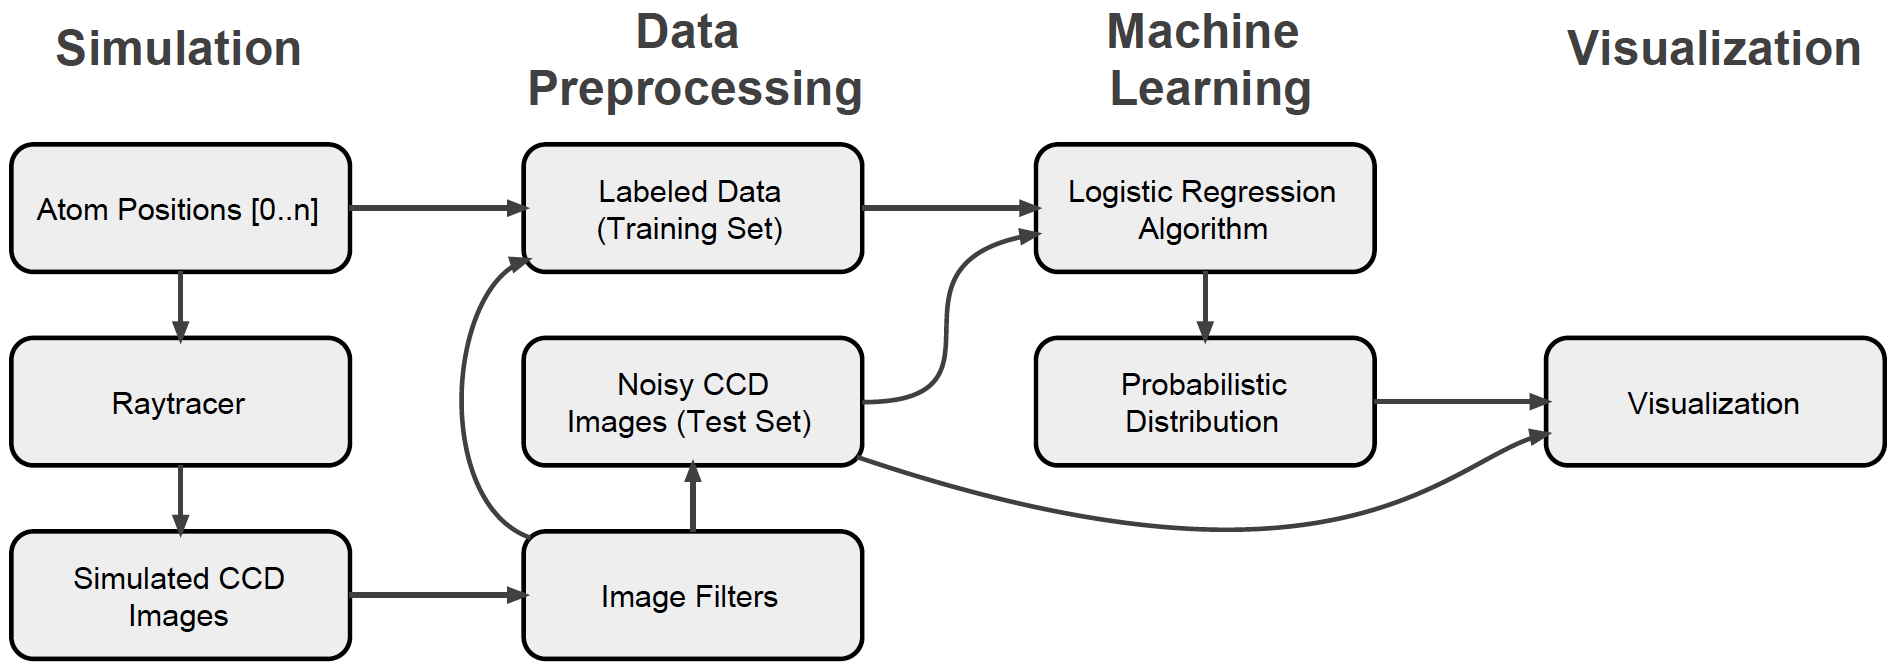
\includegraphics[scale=0.4]{arch.png}
  \caption{Clean training image.}
  \label{fig:sub1}
\end{subfigure}%
\begin{subfigure}{.5\textwidth}
  \centering
  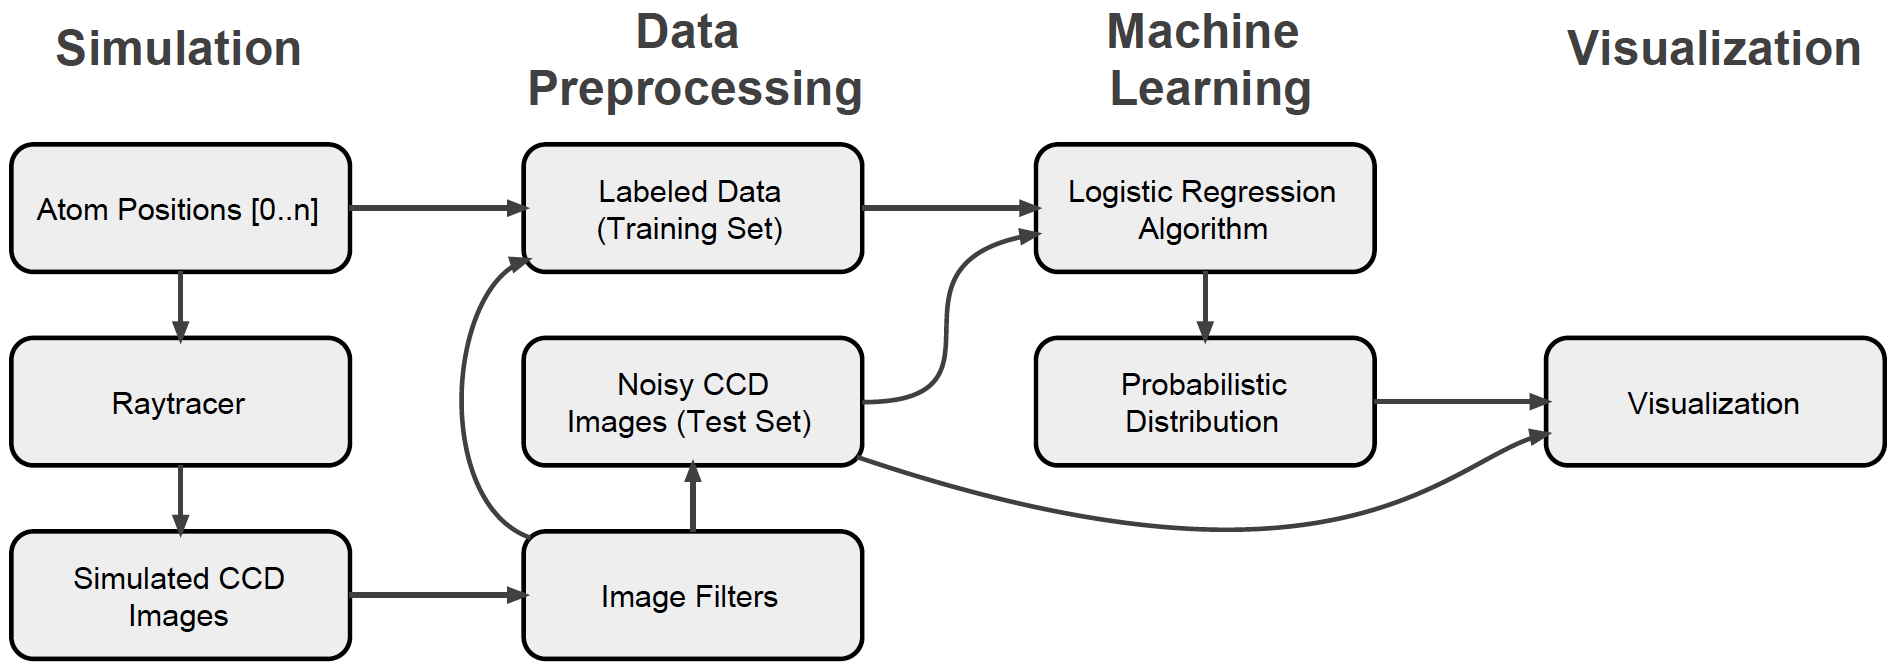
\includegraphics[scale=0.4]{arch.png}
  \caption{Noise testing image.}
  \label{fig:sub2}
\end{subfigure}
\caption{Traing and testing image examples.}
\label{fig:test}
\end{figure}

\end{frame}

\section{Design}

\begin{frame}{Design and Objective}

\begin{figure}[h]
\begin{center}
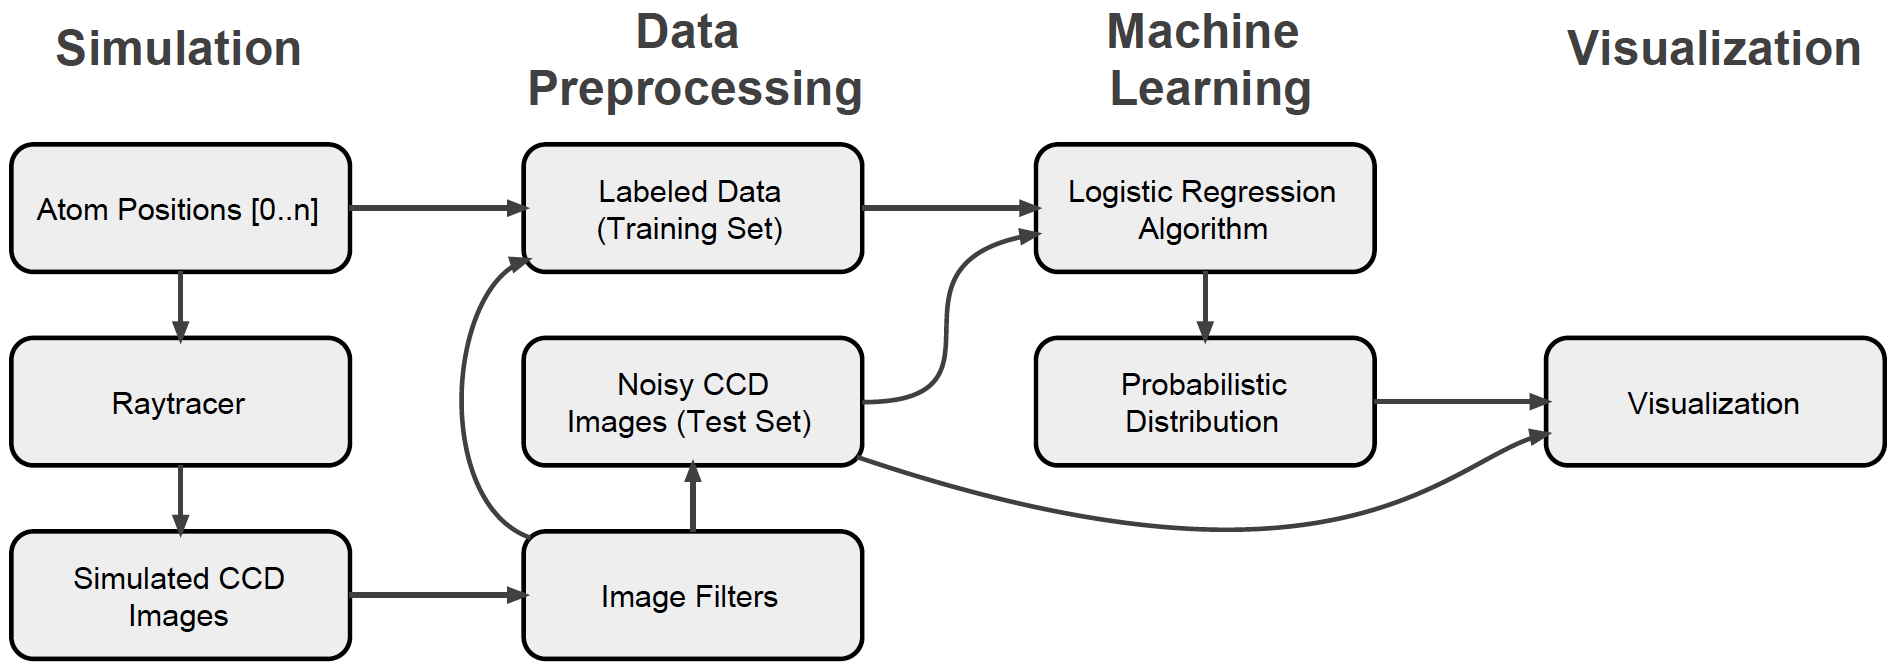
\includegraphics[scale=0.32]{arch.png}
\caption{High Level Data Flow Architecture Diagram}
\label{fig:small}
\end{center}
\end{figure}

\textbf{Objective:} Create and test a scalable machine learning solution for atom location prediction using CCD images.

\end{frame}


\section{Development}

\begin{frame}{Development and Implementation}

Our development efforts are divided into sections based on our data flow architecture with some overlap of effort in the data preprocessing step.\\

\vspace{.3cm}
\textbf{4 Development Directions:}
\begin{itemize}
\item Simulation
\item Data Preprocessing
\item Machine Learning
\item Visualization
\end{itemize}

\end{frame}

\begin{frame}{Simulation}

\textbf{Raytracer Development}
\begin{itemize}
\item Basic Raytracer -- vector operations, surface definition, refraction
\item Imaging System
\end{itemize}

\begin{figure}
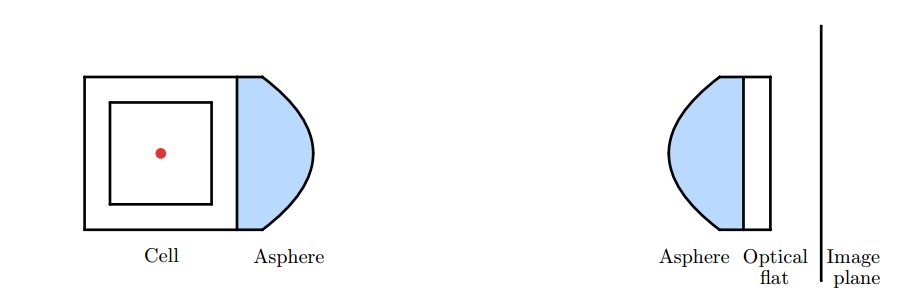
\includegraphics[scale=0.3]{asphere.png}
\caption{Scale model of the atom imaging system.}
\end{figure}

\end{frame}

\begin{frame}{Simulation}

\begin{figure}
\centering
\begin{subfigure}{.5\textwidth}
  \centering
  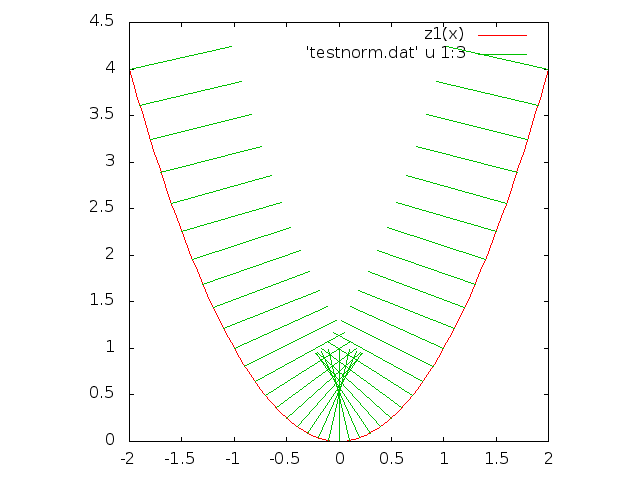
\includegraphics[scale=.3]{out.png}
  \caption{A norm}
  \label{fig:sub1}
\end{subfigure}%
\begin{subfigure}{.5\textwidth}
  \centering
  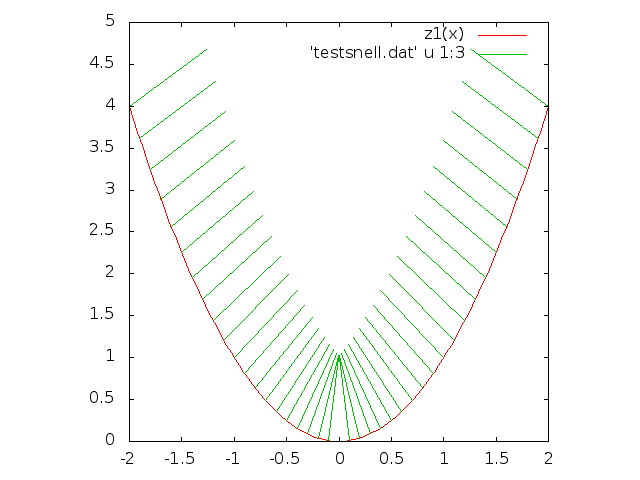
\includegraphics[scale=.3]{out2.png}
  \caption{A snell}
  \label{fig:sub2}
\end{subfigure}
\label{fig:test}
\end{figure}


\end{frame}

\begin{frame}{Simulation}
\begin{figure}
\centering
\begin{subfigure}{.5\textwidth}
  \centering
  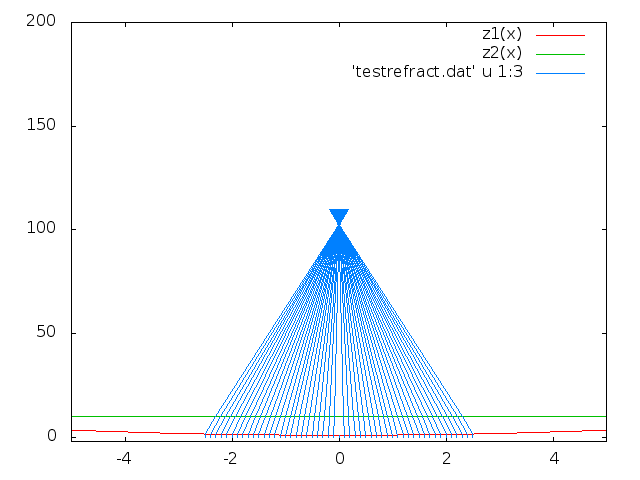
\includegraphics[scale=.3]{out4.png}
  \caption{A refract}
  \label{fig:sub3}
\end{subfigure}%
\begin{subfigure}{.5\textwidth}
  \centering
  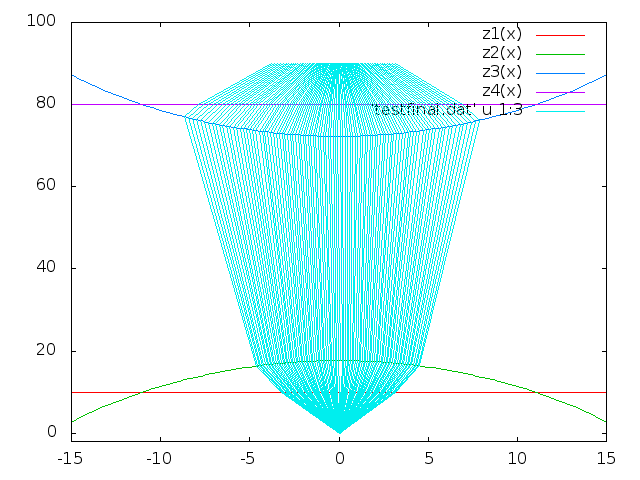
\includegraphics[scale=.3]{out5.png}
  \caption{A lenstest}
  \label{fig:sub4}
\end{subfigure}
\label{fig:test2}
\end{figure}

\end{frame}


\begin{frame}{Data Preprocessing}

\textbf{4 Directions for Data Preprocessing:}
\begin{itemize}
\item Filtering
\item Noise Adding
\item Data Partitioning
\item Feature Scaling
\end{itemize}

\end{frame}

\begin{frame}{Machine Learning}

\begin{itemize}
\item \textbf{Spark} -- 
\item \textbf{HaLoop} -- 
\item \textbf{Twister} -- 
\end{itemize}

\end{frame}

\begin{frame}{Data Visualization}

\begin{itemize}
\item \textbf{Spark} -- 
\item \textbf{HaLoop} -- 
\item \textbf{Twister} -- 
\end{itemize}

\end{frame}


\section{Lessons Learned}

\begin{frame}{Lessons Learned}
\textbf{Simulation}
\begin{itemize}

\end{itemize}

\textbf{Data Preprocessing}
\begin{itemize}

\end{itemize}

\textbf{Machine Learning}
\begin{itemize}

\end{itemize}

\textbf{Data Visualization}
\begin{itemize}

\end{itemize}

\end{frame}


\section{Conclusion}

\begin{frame}{Conclusion}

\begin{itemize}
\item \textbf{Percolator} -- Developed by Google to replace MapReduce.  Updates only a portion of PageRank indices by propagating the influence of new, or altered, web pages.
\item \textbf{Pregel} -- A general framework for superstep-based graphical updates.  Allows for dynamic changes to graph structure.
\item \textbf{Ceil} -- Uses runtime analysis of dependency graphs to dynamically optimize execution.  Runtime analysis allows for detection of iterative/recursive patterns.
\item \textbf{Flumejava} -- Preprocesses execution plan to generate a DAG, which is used to perform fusion-based optimizations.
\end{itemize}

\end{frame}


%------------------------------------------------

\begin{frame}
\Huge{\centerline{The End}}
\end{frame}

%---------------------------------------------------------------------------------------

%\begin{frame}[allowframebreaks]{References}
%\begin{small}
%\bibliographystyle{plainnat}
%\bibliography{references}
%\end{small}
%\end{frame}

\end{document} 